\documentclass[11pt]{article}
\usepackage[utf8]{inputenc}
\usepackage[T1]{fontenc}
\usepackage{grffile}
\usepackage{longtable}
\usepackage{wrapfig}
\usepackage{rotating}
\usepackage[normalem]{ulem}
\usepackage{amssymb,amsmath,amsthm}
\usepackage{textcomp}
\usepackage{amssymb}
\usepackage{capt-of}
\usepackage{hyperref}
\hypersetup{colorlinks=true, linkcolor=magenta, citecolor=cyan}
\setlength{\parindent}{0in}
\usepackage[margin=1in]{geometry}
\usepackage[english]{babel}
\usepackage{mathtools}
\usepackage{palatino}
\usepackage{fancyhdr}
\usepackage{sectsty}
\usepackage{engord}
\usepackage{parskip}
\usepackage{minted}
\usepackage{graphicx}
\usepackage{subcaption}
\usepackage{setspace}
\usepackage{placeins}
\usepackage{color}
\usepackage{bm}
\usepackage{pdfpages}
\usepackage{natbib}

\usepackage{graphicx} % Inclusión de imágenes.
\usepackage{grffile}  % Distintos formatos para imágenes.
\usepackage{longtable} % Tablas multipágina.
\usepackage{wrapfig} % Coloca texto alrededor d

\theoremstyle{definition}

% Tikz
\usepackage{tikz}
\usetikzlibrary{positioning}
\usetikzlibrary{bayesnet}
\usetikzlibrary{shapes.geometric}
\usetikzlibrary{decorations.text}

\author{Luis Antonio Ortega Andrés}
\date{\today}
\title{Bayesian methods}

\newcommand*{\QED}{\null\nobreak\hfill\ensuremath{\square}}%

\begin{document}

\maketitle

This document contains notes and exercises done during the course of Bayesian methods. All the following theory is explained from a non-variational point of view, this includes the EM algorithm.

\section{Introduction to Bayesian networks}

Given a set of variables \(\bm{X} = (X_{1},\dots,X_{N})\), \emph{Bayesian networks} might be defined either as a probability distribution of a certain form or a DAG whose nodes represent these variables and links an independence constraint. Both ideas are present in the following definition.

\textbf{Definition}. A \emph{belief network or Bayesian network} is a pair \((G,P)\) formed by a DAG \(G\) and  joint probability distribution \(P\) such that there is a correspondence between variables and nodes verifying:
  \[
    P(x_{1},\dots,x_{N}) = \prod_{n=1}^{N}P(x_{n}\mid pa(x_{n})).
  \]

\textit{Remark}. A Bayesian network might be given as a distribution from which the DAG can be constructed or a DAG which represents the distribution. For example in Figure~\ref{fig:bn_example}, given the DAG one could easily define the joint distribution and conversely.


\begin{figure}[h!]
  \centering
  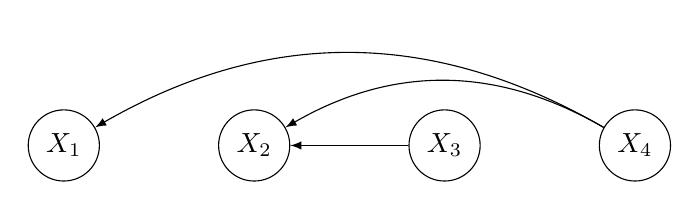
\begin{tikzpicture}[
    node distance=1.5cm and 1.5cm,
    mynode/.style={draw,circle,text width=0.5cm,align=center}
    ]

    \node[mynode] (1) {\(X_1\)};
    \node[mynode,right=of 1] (2) {\(X_2\)};
    \node[mynode,right=of 2] (3) {\(X_3\)};
    \node[mynode,right=of 3] (4) {\(X_4\)};

    \path (4) edge[-latex][bend right] (1)
    (3) edge[-latex] (2)
    (4) edge[-latex][bend right] (2)
    ;

    \end{tikzpicture}
    \captionof{figure}{Bayesian Network factorizing \(P(x_1, x_2, x_3, x_4) = P(x_1 \mid x_4)P(x_2\mid x_3, x_4)P(x_3)P(x_4)\).}\label{fig:bn_example}
\end{figure}

Any probability distribution can be written as a Bayesian network, even though it may end up being a fully-connected ``cascade''\footnote{This term comes from the visual structure of the graph.} DAG, which means that each variable \( X_n \) is a parent of any \( X_m \) with \( m > n \). This is because any distribution satisfies:
\[
   P(x_1, \dots, x_{N}) = P(x_1) \prod_{n=2}^{N}P(x_{n} \mid x_{1},\dots, x_{n-1})
 \]


 
\subsection{D-separation and D-connection}

There are two central concepts that determine conditional independence in any Bayesian network, these are \emph{d-connection} and \emph{d-separation}.

\textbf{Definition}. Let \(G\) be a DAG where \(\bm{X}, \bm{Y} \text{ and } \bm{Z}\)
  are disjoint sets of vertices. We say that \(\bm{X} \text{ and
  } \bm{Y}\) are \emph{d-connected} by \(\bm{Z}\) if and only if there
  exists an undirected path \(U\) from any vertex in \(\bm{X}\) to any
  vertex in \(\bm{Y}\) such that:
  \begin{itemize}
    \item For any  collider \(C\), itself or any it's descendants is in \(\bm{Z}\).
    \item No non-collider on \(U\) is on \(\bm{Z}\).
  \end{itemize}
  That is, there exists a path where \(\bm{Z}\) contains all of its colliders and their descendants, and no other node from the path.


\textbf{Definition}. Let \(G\) be a DAG where \(\bm{X}, \bm{Y} \text{ and } \bm{Z}\) are disjoint sets of vertices. \(\bm{X}\) and \(\bm{Y}\) are \emph{d-separated} by \(\bm{Z}\) if and only if they are not d-connected by \(\bm{Z}\) in \(G\). That is, for any undirected path from \(\bm{X}\) to \(\bm{Y}\), either there is a collider or a descendant of it not in \(\bm{Z}\) or there is a non-collider in  \(\bm{Z}\).

\begin{figure}[t]
\centering
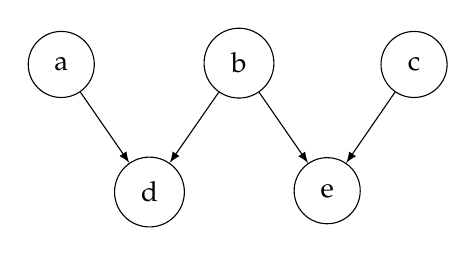
\begin{tikzpicture}[
  node distance=1cm and 0.5cm,
  mynode/.style={draw,circle,text width=0.5cm,align=center}
]

\node[mynode] (a) {a};
\node[mynode, below right=of a] (d) {d};
\node[mynode,above right=of d] (b) {b};
\node[mynode, below right=of b] (e) {e};
\node[mynode,above right=of e] (c) {c};

\path (a) edge[-latex] (d)
(b) edge[-latex] (d)
(c) edge[-latex] (e)
(b) edge[-latex] (e)
;

\end{tikzpicture}
\caption{D-separation example}\label{fig:d-sep}
\end{figure}

For example, in Figure~\ref{fig:d-sep}, \(d\) d-separates \(a\) and \(c\) (\(e\)
is a collider in the path that is not in \(\{d\}\)),
and \(\{d,e\}\) d-connect them.

\textbf{Theorem} (\cite{spirtes2000causation}, Th 3.3). Let \(G\) be a DAG where \(\bm{X}, \bm{Y} \text{ and } \bm{Z}\)
are disjoint sets of vertices. \(\bm{X}\) and \(\bm{Y}\)
are d-separated by \(\bm{Z}\) if and only if they are independent conditional
on \(\bm{Z}\) in all probability distributions that \(G\) may represent.


In cases where the Bayesian networks contains i.i.d nodes that are
essentially the same but repeated a number of times, the \emph{plate notation} is commonly used to represent this nodes in a compacted format (Figure~\ref{fig:plate_notation}).

\begin{figure}[t]
\centering
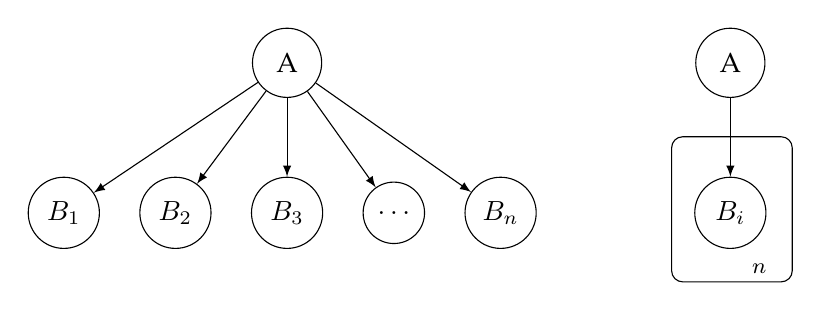
\begin{tikzpicture}[
  node distance=1cm and 0.5cm,
  mynode/.style={draw,circle,text width=0.5cm,align=center}
]

\node[mynode] (a) {A};
\node[mynode,below=of a] (d) {\(B_3\)};
\node[mynode,left=of d] (c) {\(B_2\)};
\node[mynode,left=of c] (b) {\(B_1\)};
\node[mynode,right=of d] (e) {\(\dots\)};
\node[mynode,right=of e] (f) {\(B_n\)};

\node[mynode,right=2cm of f] (g) {\(B_i\)};
\node[mynode, above=of g] (h) {A};
\plate[inner sep=.3cm,xshift=.02cm,yshift=.2cm]  {} {(g)} {\(n\)}; %


\path (a) edge[-latex] (b)
(a) edge[-latex] (c)
(a) edge[-latex] (d)
(a) edge[-latex] (e)
(a) edge[-latex] (f)
(h) edge[-latex] (g)
;

\end{tikzpicture}
\caption{Plate notation example. Standard notation on the left and plate on the right.}\label{fig:plate_notation}
\end{figure}


\section{Maximum likelihood learning in Bayesian networks}

Given a parameterized model, that is, a set of variables \( X_1,\dots,X_N \) given that their distribution is governed by a set of parameters \( \Theta \). Maximum likelihood estimation consists on, given a set of observations \( \mathcal{D} \), find
\[
   \Theta^{ML} = argmax_{\Theta} \mathcal{L}(\Theta, \mathcal{D}) =  argmax_{\Theta} P(\mathcal{D} \mid \Theta).
\] 
In simple cases, this can be approached deriving the corresponding expression and finding those minimals analytically. In this section we are reviewing this exact approach in Bayesian networks.

Consider a scenario where a disease \(D\) and two habits \(A\) and \(B\) are being studied.  Consider the following i.i.d variables \(\{A_{1},\dots, A_{N}\}\), \(\{B_{1},\dots,B_{N}\}\) and \(\{D_{1},\dots, D_{N}\}\) governed by the parameters \(\theta_{A}, \theta_{B}\) and \(\bm{\theta}_{D}\) as shown in figure~\ref{fig:bayesian_example}. Let \(N = 7\) be the number of observations of the variables as shown in Table~\ref{tab:bn_ex} and \( \bm{x} = \{(a_n, b_n, d_n),\ n=1,\dots,N\} \) the set of observations.

All the variables are binary satisfying
\[
  P(A_{n} = 1 \mid \theta_{A}) = \theta_{A}, \quad P(B_{n} = 1 \mid \theta_{B}) = \theta_{B} \quad \forall n=1,\dots,N,
\]
\[
  P(D_{n} = 1 \mid A_{n} = 0, B_{n} = 1, \bm{\theta}_{D}) = \theta_{1}, \quad \forall n = 1,\dots,N,
\]
\[
  \bm{\theta}_{D} = ( \theta_{0}, \theta_{1}, \theta_{2}, \theta_{3}).
\]
Where a binary to decimal transformation between the states of \(A\) and \(B\) and the sub-index of \(\theta\) is being used.

\begin{figure}[H]
  \centering
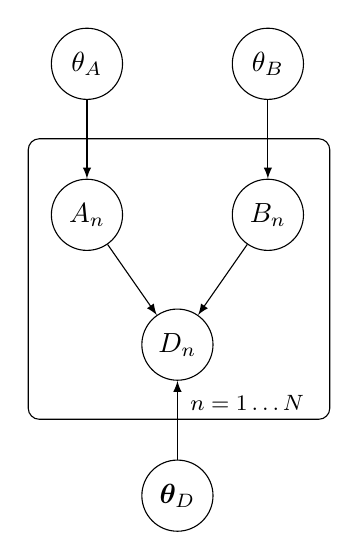
\begin{tikzpicture}[
  node distance=1cm and 0.5cm,
  mynode/.style={draw,circle,text width=0.5cm,align=center}
]

  \node[mynode] (d) {\(D_{n}\)};
  \node[mynode, above left=of d] (a) {\(A_{n}\)};
  \node[mynode, above right=of d] (b) {\(B_{n}\)};
  \node[mynode, above=of a] (ta) {\(\theta_{A}\)};
  \node[mynode, above=of b] (tb) {\(\theta_{B}\)};
  \node[mynode, below=of d] (td) {\(\bm{\theta}_{D}\)};
  \plate[inner sep=.3cm,xshift=.02cm,yshift=.2cm]  {} {(d)(a)(b)} {\(n= 1\dots N\)}; %
  \path (a) edge[-latex] (d)
        (b) edge[-latex] (d)
        (ta) edge[-latex] (a)
        (tb) edge[-latex] (b)
        (td) edge[-latex] (d)
  ;
\end{tikzpicture}
\caption{Bayesian network of disease example}\label{fig:bayesian_example}
\end{figure}


The graph gives the following joint probability distribution the variables:
\[
P(a_{n},b_{n},d_{n}, \theta_A, \theta_B, \theta_D) = P(d_{n}\mid a_{n},b_{n},\theta_D)P(a_{n} \mid \theta_A)P(b_{n} \mid \theta_A).
\]
A prior distribution must be specified and since dealing with multidimensional continuous
distributions is computationally problematic, it is usual to use uni-variate
distributions.

\subsection{Learning binary variables}

The simplest cases to continue are \(P(\theta_{A} \mid \bm{x}_{A})\) and
\(P(\theta_{B} \mid \bm{x}_{B})\) since they require only a uni-variate prior distribution
\(P(\theta_{A})\) or \(P(\theta_{B})\). The procedure is shown using \( \theta_A \) and it is analogous when using \( \theta_B \). 

The posterior is
\[
  P(\theta_{A} \mid \bm{x}_{A}) = \frac{1}{P(\bm{x}_{A})}P(\theta_{A})\theta_{A}^{\#(A=1)}{(1-\theta_{A})}^{\#(A=0)}.
\]
The most convenient choice for the prior is a Beta distribution as conjugacy
will hold:
\[
  \theta_{A} \sim \text{Beta}(\alpha_{A}, \beta_{A}) \implies P(\theta_{A})  = \frac{1}{B(\alpha_{A}, \beta_{A})}\theta_{A}^{\alpha_{A}-1}(1-\theta_{A})^{\beta_{A} - 1}.
\]
Therefore, it follows that
\[
  \theta_{A} \mid \bm{x}_{A} \sim \text{Beta}(\alpha_{A} + \#(A=1), \beta_{A} + \#(A = 0)).
\]

The predictive marginal is then
\[
  \begin{aligned}
    P(A = 1 \mid \bm{x}_{A})
    &= \frac{P(A = 1, \bm{x}_{A})}{P(\bm{x}_{A})} = \int_{\theta_{A}}  \frac{P(A = 1, \bm{x}_{A}, \theta_{A})}{P(\bm{x}_{A})} =  \int_{\theta_{A}}  \frac{P(A = 1 \mid \bm{x}_{A}, \theta_{A}) P(\bm{x}_{A}, \theta_{A})}{P(\bm{x}_{A})} \\
    &=  \int_{\theta_{A}}  \frac{P(A = 1 \mid \bm{x}_{A}, \theta_{A}) P(\theta_{A} \mid \bm{x}_{A})P(\bm{x}_{A})}{P(\bm{x}_{A})} \\
    &= \int_{\theta_{A}}P(\theta_{A}\mid \bm{x}_{A})\theta_{A} = \mathbb{E}[\theta_{A} \mid \bm{x}_{A}] \\
    &= \frac{\alpha_{A} + \#(A= 1)}{\alpha_{A} + \#(A=1) + \beta_{A} + \#(A=0)}.
  \end{aligned}
\]
Where the last equality is given by the expected value of a Beta distribution.

For \(P(d \mid a ,b)\) the situation is more complex, the simplest approach
is to specify a Beta prior for each of the components of \(\bm{theta}_{D}\).
Focus on \(\theta_{2}\), notice the parameters \(\alpha\)
and \(\beta\) we used before now do depend on \(A\) and \(B\):
\[
  \theta_{2} \sim Beta\Big(\alpha_{D}(1,0) + \#(D = 1, A = 1, B = 0), \ \beta_{D}(1,0) + \#(D = 0, A = 1, B = 0)\Big).
\]

Repeating the procedure we used with \(A\) we get that
\[
  P(D = 1 \mid A = 1, B = 0, \bm{x}) = \frac{\alpha_{D}(1,0) + \#(D = 1, A = 1, B = 0)}{\alpha_{D}(1,0) + \beta_{D}(1,0) + \#(A=1, B = 0)}.
\]

All hyperparameters could be set to the same
value, where a complete ignorance prior would correspond to set them to 1.

There are two limit possibilities depending on the amount of data available.
\begin{itemize}
  \item \textbf{No data}. The marginal probability corresponds to the prior, which
in the last case is
    \[
    P(D = 1 \mid A = 1, B = 0, \bm{x}) = \frac{\alpha_{D}(1,0)}{\alpha_{D}(1,0) + \beta_{D}(1,0)}.
    \]
    Note that equal hyperparameters would give a result of \(0.5\).\newline
   
  \item \textbf{Infinite data}. When infinite data is available, the marginal is generally dominated by it,
    this corresponds to the Maximum Likelihood solution.
    \[
    P(D = 1 \mid A = 1, B = 0, \bm{x}) = \frac{\#(D = 1, A = 1 , B = 0)}{\#(A = 1, B = 0)}.
    \]
    This happens unless the prior has a pathologically strong effect.
\end{itemize}

\begin{figure}
  \centering
  \begin{tabular}{ccc}
\hline
  A & B & D \\ \hline
  \(1\) & \(1\) & \(1\) \\
  \(1\) & \(0\) & \(0\) \\
  \(0\) & \(1\) & \(1\) \\
  \(0\) & \(1\) & \(0\) \\
  \(1\) & \(1\) & \(1\) \\
  \(0\) & \(0\) & \(0\) \\
  \(1\) & \(0\) & \(1\) \\ \hline
\end{tabular}
\caption{Set of observations, where \(1\) means true and \(0\) means false.}\label{tab:bn_ex}
\end{figure}

 Consider the data given in the table in figure \ref{fig:bayesian_example}, and
 equal parameters and hyperparameters \(1\) and a prior belief that any setting is equally probable, i.e, \( P(A=1) = 0.5\) . 
 
 We may illustrate the different results that are obtained using using Bayesian inference and Maximum likelihood training. The former is
 \[
   P(A = 1 \mid \bm{x}) = \frac{1 + \#(A = 1)}{2 + N} = \frac{5}{9} \approx 0.556.
 \]
 and the latter is \(4/7 = 0.571\). In conclusion, the Bayesian
 result is more prudent than this one, which fits in with our prior belief.

\subsection{Frequentist vs Bayesian}

The main disadvantages of frequentist approaches are:
\begin{enumerate}
  \item They assign zero probability to events just because they do not appear in the considered sample.
  \item They only consider the ratio of the outcomes but not their amount.
\end{enumerate}

\subsection{Missing data}

There are situations where maximum likelihood estimation cannot be approached as we have done before, for example, when there is missing data or latent (unobserved) variables.

There are three types of missing data:
\begin{enumerate}
  \item \textbf{Missing completely at random}: The reason why those values are missing is independent of the values themselves and the observed ones.
  \item \textbf{Missing at random}: The fact that data is missing is not completely random but can be explained given the observed ones.
  \item \textbf{Missing not at random}: The reason why data is missing is related with such data.
\end{enumerate}

Consider the following example with missing data: let \( X, Y \) be two random variables such that
\[
   P(x, y \mid \Theta) = P(x \mid \theta_x)P(y \mid x, \theta_{y\mid x}) = \theta_x \ \theta_{y\mid x}.
\]
That is, we are considering a simple Bayesian network \( X \to Y \), with both variables being bernoulli trials. Consider the following set of observations \( \mathcal{D} = \{(?, y_0)), (x_0, y_1), (?, y_0) \). The likelihood is
\[
   \mathcal{L}(\Theta, \mathcal{D}) = P(y_0)^2P(x_0, y_1) = P(y_1 \mid x_0)P(x_0)\left(\sum_x P(y_0\mid x)P(x)\right)^2 = (\theta_{x_0}\theta_{y_0 \mid x_0} + \theta_{x_1}\theta_{y_0 \mid x_1} )^2 \theta_{x_0}\theta_{y_1 \mid x_0}.
\]  
Where its partial derivatives cannot be independently optimized. 

\subsection{EM algorithm}
The EM algorithm performs maximum likelihood estimation in probabilistic models with missing data. Its main idea is to follow a two-step iterative process where, the first computes the expected value of the missing data and the second optimized the set of parameters.




\clearpage
\nocite{*}
\bibliographystyle{authordate1}
\bibliography{refs}

\end{document}